%====================================================================================
\section[Contrato]{Curva de contrato}
%====================================================================================

%------------------------------------------------
\begin{frame}{Optimo de Pareto}
	Para un determinado tamaño de caja , ¿ donde están todas las asignaciones
	óptimo paretianas o pareto eficientes
\end{frame}
%------------------------------------------------
\begin{frame}{Efficiencia en el intercambio}
	\begin{itemize}
		\item La curva de contrato
			\begin{itemize}
				\item Para encontrar todas las asignaciones eficientes de ropa y alimentos entre Karen y Jaime, se deben buscar todos los puntos de tangencia entre sus curvas de indiferencia.
				\item La \textbf{curva de contrato} muestra todas las asignaciones eficientes entre dos agentes económicos. Es independiente de las dotaciones individuales. Rasgo geométrico: las relaciones marginales de sustitución son iguales.
				\item Para calcular la curva de contrato se maximiza la utilidad de un agente sujeta a las restricciones de factibilidad y de utilidad del otro agente.
			\end{itemize}
	\end{itemize}
\end{frame}
%------------------------------------------------
\begin{frame}{La curva de contrato o Conjunto paretiano}
		Los puntos Pareto Eficiente son $F$, $E$ y $G$\\
		\vspace{-0.6cm}
	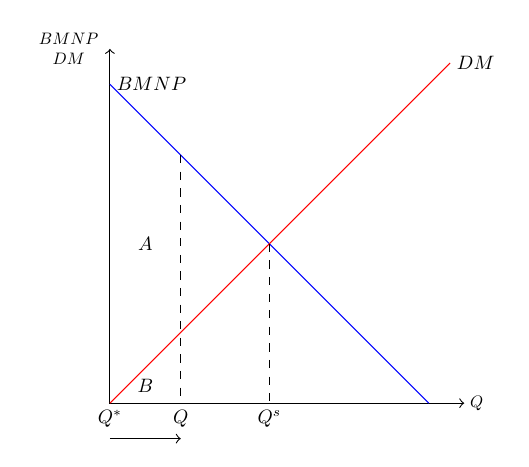
\begin{tikzpicture}[scale=0.9]
% Ejes
\draw[<->] (0,5)  node [text width=15mm,text centered, scale=0.6, left] {$BMNP$ $DM$}-- (0,0) -- (5,0) node [scale=0.6, right] {$Q$};

% Rectas
\draw[blue] (0,4.5) node [right, scale=0.7, black] {$BMNP$} -- (4.5,0);
\draw[red] (0,0)  node [below, scale=0.7, black] {$Q^\ast$} -- (4.8,4.8) node [right, scale=0.7, black] {$DM$};

% Rectas sombreadas
\draw[dashed] (1,3.5) -- (1,0)  node [below, scale=0.7, black] {$Q$};
\draw[dashed] (2.25, 2.25) -- (2.25,0) node [below, scale=0.7, black] {$Q^s$};

% A y B
\draw (0.5,2.25) node [scale=0.7, black] {$A$};
\draw (0.5,0.25) node [scale=0.7, black] {$B$};

% Flechas
\draw[->] (0,-0.5) -- (1,-0.5);
\end{tikzpicture}
\end{frame}
%------------------------------------------------
\begin{frame}{Casos especiales}
	Para A: bienes complementos perfectos\\
	Para B: bienes sustitutos perfectos
		$$u^{A}=\text{min}(x_{1}^{A},x_{2}^{A}) \quad ; \quad u^{B}=ax_{1}^{B}+bx_{2}^{B}$$\\
			\centering
		\begin{tikzpicture}[domain=5:10,
	tangent/.style={
		decoration={
			markings,% switch on markings
			mark=
			at position #1
			with
			{
				\coordinate (tangent point-\pgfkeysvalueof{/pgf/decoration/mark info/sequence number}) at (0pt,0pt);
				\coordinate (tangent unit vector-\pgfkeysvalueof{/pgf/decoration/mark info/sequence number}) at (1,0pt);
				\coordinate (tangent orthogonal unit vector-\pgfkeysvalueof{/pgf/decoration/mark info/sequence number}) at (0pt,1);
			}
		},
		postaction=decorate
	},
	use tangent/.style={
		shift=(tangent point-#1),
		x=(tangent unit vector-#1),
		y=(tangent orthogonal unit vector-#1)
	},
	use tangent/.default=1,
	transform canvas={scale=0.5}
	]       
	% Curva
	\draw[white, samples=1000, tangent=0.4] plot (\x, {sqrt(10-\x)/0.5 });
	% Relleno
	\fill [pattern=crosshatch dots,pattern color=green!60!white] (5,4.74) -- (10,1.6) -- (10,0) -- (5,0) -- (5,6);
	% Ejes
	\draw[<->] (4,0) node[align=center, left, scale=0.8] {$-L$} -- (10,0) node[align=center, below] {\footnotesize $O_L$} -- (10,5) node[align=center, above, scale=0.8] {$q$};
	\draw[<->] (5,5) node[align=center, above, scale=0.8] {$c$} -- (5,0) node[align=center, below, scale=0.8] {$O_R$} -- (11,0) node[align=center, right, scale=0.8] {$R$};
	% Tangente - Punto
	\draw[use tangent] (-2.92,0) -- (4,0);
	\filldraw[use tangent] (0,0) circle (2pt) node[align=center, above right, scale=0.8] {$M$};
	% Flechas
	\draw[<->] (5,-0.5) -- (7.5,-0.5) node[align=center, below, scale=0.8] {$\overline{L}$} -- (10,-0.5);
	% Curvas de indiferencia
	\draw [smooth,blue,thick] (5.8,5) to[out=299, in=161] (9.8,2.2);
	% Linea punteadas
	\draw[dashed] (7.48,0) node [scale=0.8, below] {$R(p,w)$} -- (7.48,3.18) -- (5,3.18) node [scale=0.8, left] {$c(p,w)$};
	% Felcha
	\draw[->] (10.5,2.1) node [scale=0.8, right] {$\frac{\pi(p,w)}{p}$} -- (10,1.6);
	% Etiqueta de pendiente
	\draw (10.9,0.9) node [scale=0.8, right] {$m = \frac{w}{p}$};
	
\end{tikzpicture}
\end{frame}
%------------------------------------------------
\begin{frame}{Casos especiales}
	Para A: bienes complementos perfectos \\
	Para B: bienes sustitutos imperfectos
		$$u^{A}=\text{min}(x_{1}^{A},x_{2}^{A}) \quad ; \quad u^{B}=ax_{1}^{B}x_{2}^{B}$$\\
			\centering
		\begin{tikzpicture}
	% Formato de CAJA
	\draw[->] (0.5,0.5) node[align=center, below left] {\footnotesize $O_A$} -- (0.5,4.5) node[align=center, above] {\footnotesize $x_{2}^{A}$};
	\draw[->] (0.5,0.5) -- (8.5,0.5) node[align=center, right] {\footnotesize $x_{1}^{A}$};
	
	\draw[->] (8,4) node[align=center, above right] {\footnotesize $O_B$} -- (0,4) node[align=center, left] {\footnotesize $x_{2}^{B}$};
	\draw[->] (8,4) -- (8,0) node[align=center, below] {\footnotesize $x_{2}^{B}$};
	
	% Curvas de indiferencia1
		% Agente A1
			\draw [blue] (1.51,3.5) --  (1.51,1.14) -- (4.01,1.14);
			\draw [blue] (2.82,3.5) -- (2.82,1.98) --  (4.4,1.98);
			\draw [blue] (4.28,3.5) --  (4.28,2.91) -- (4.9,2.91);
			
		% Agente B
			\draw  [red] (0.6,1.5) ..controls (1.4,1.4) and (1.74,1) .. (2,0.55);
			\draw  [red] (1.6,2.5) ..controls (2.4,2.4) and (3,2) .. (3.3,1.2);
			\draw  [red] (3.2,3.5) ..controls (3.7,3.4) and (4.3,3.2) .. (4.8,2.1);
			
		% Curva de contrato
			\draw [purple] (0.5,0.5) -- (6,4);
			
		% Puntos
			\draw[black, fill=black] (1.51,1.14) circle[radius=0.04];
			\draw[black, fill=black] (2.82,1.98) circle[radius=0.04];
			\draw[black, fill=black] (4.28,2.91) circle[radius=0.04];
	
	% Flechas
		\node[draw, single arrow,
				minimum height=21mm, minimum width=1mm,
				single arrow head extend=1.5mm,
				anchor=west, blue, fill=blue, scale=0.5, rotate=33] at (1.7,2.7) {};
		\node[draw, single arrow,
				minimum height=28mm, minimum width=1mm,
				single arrow head extend=1.5mm,
				anchor=west, red, fill=red, rotate=-147, scale=0.5] at (4.5,2.3) {};
		
		% Conjunto paretiano
			\node[draw, single arrow,
					minimum height=22mm, minimum width=1mm,
					single arrow head extend=1.5mm,
					anchor=west, purple, scale=0.5, rotate=180,transform shape] at (7.2,3.5) {\rotatebox {180} { \small Conjunto paretiano}};
\end{tikzpicture}
\end{frame}
%------------------------------------------------
\begin{frame}{Casos especiales}
	Para A y B: bienes complementos perfectos
	$$u^{A}=\text{min}(x_{1}^{A},x_{2}^{A}) \quad ; \quad u^{B}=\text{min}(x_{1}^{B},x_{2}^{B})$$\\
		\centering
	\begin{tikzpicture}
	% Formato de CAJA
		\draw[->] (0.5,0.5) node[align=center, below left] {\footnotesize $O_A$} -- (0.5,4.5) node[align=center, above] {\footnotesize $x_{2}^{A}$};
		\draw[->] (0.5,0.5) -- (8.5,0.5) node[align=center, right] {\footnotesize $x_{1}^{A}$};
		
		\draw[->] (8,4) node[align=center, above right] {\footnotesize $O_B$} -- (0,4) node[align=center, left] {\footnotesize $x_{2}^{B}$};
		\draw[->] (8,4) -- (8,0) node[align=center, below] {\footnotesize $x_{2}^{B}$};
	
	% Curvas de indiferencia1
		% Agente A1
			\draw [blue] (1.51,2) --  (1.51,1.14) -- (2.4,1.14);
			\draw [blue] (2.82,2.84) -- (2.82,1.98) --  (3.71,1.98);
			\draw [blue] (4.28,3.77) --  (4.28,2.91) -- (5.17,2.91);
		% Agente B 0.93
			\draw [red] (3.06,1.45) --  (3.99,1.45) -- (3.99,0.59);
			\draw [red] (4.36,2.27) --  (5.29,2.27) -- (5.29,1.41);
			\draw [red] (5.74,3.16) --  (6.67,3.16) -- (6.67,2.3);
			
	% Curva de contrato
		\draw [purple] (0.5,0.5) -- (6,4);
		\draw [purple] (8,4) -- (2.5,0.5);
			% Rellenando la curva de contrato
				\fill [pattern=crosshatch dots,pattern color=purple!30!white](0.5,0.5)--(6,4)--(8,4)--(2.5,0.5)--(0.5,0.5);
			% Conjunto paretiano
				\node [scale=0.15mm]  at (6.7, 3.8)  {\textbf{Conjunto paretiano}};
\end{tikzpicture}
\end{frame}
%------------------------------------------------
\begin{frame}{Casos especiales}
	Para A y B: un mismo bien es neutral
	$$u^{A}=ax_{1}^{A} \quad ; \quad u^{B}=x_{1}^{B}$$\\
	\vspace{3cm}
		\input{tikzs/fig_12}
\end{frame}
%------------------------------------------------
\begin{frame}{Casos especiales}
	Para A: bien $x_2$ es neutral \\
	Para B: bien $x_1$ es neutral
	$$u^{A}=ax_{1}^{A} \quad ; \quad u^{B}=x_{2}^{B}$$\\
		\vspace{3cm}
	\begin{tikzpicture}[transform canvas={scale=0.6}]
	% Formato de CAJA
		\draw[->] (0.5,0.5) node[align=center, below left] {\footnotesize $O_A$} -- (0.5,4.5) node[align=center, above] {\footnotesize $x_{2}^{A}$};
		\draw[->] (0.5,0.5) -- (8.5,0.5) node[align=center, right] {\footnotesize $x_{1}^{A}$};
		
		\draw[->] (8,4) node[align=center, above right] {\footnotesize $O_B$} -- (0,4) node[align=center, left] {\footnotesize $x_{2}^{B}$};
		\draw[->] (8,4) -- (8,0) node[align=center, below] {\footnotesize $x_{2}^{B}$};
	
	% Curvas de indiferencia
		% Agente A
			\draw [blue] (1.5,3.5) -- (1.5,1);
			\draw [blue] (2,3.5) -- (2,1);
			\draw [blue] (2.5,3.5) -- (2.5,1);
		% Agente B
			\draw [red] (1,3) -- (6.5,3);
			\draw [red] (1,2.5) -- (6.5,2.5);
			\draw [red] (1,2) -- (6.5,2);
		
	% Flechas
		\node[draw, single arrow,
			minimum height=10mm, minimum width=1mm,
			single arrow head extend=1.5mm,
			anchor=west, blue, fill=blue] at (1.5,1.5) {};
		\node[draw, single arrow,
			minimum height=10mm, minimum width=1mm,
			single arrow head extend=1.5mm,
			anchor=west, red, fill=red, rotate=-90] at (6,3) {};
	
	% Formato de CAJA
		\draw[->] (10.5,0.5) node[align=center, below left] {\footnotesize $O_A$} -- (10.5,4.5) node[align=center, above] {\footnotesize $x_{2}^{A}$};
		\draw[->] (10.5,0.5) -- (18.5,0.5) node[align=center, right] {\footnotesize $x_{1}^{A}$};
		
		\draw[->] (18,4) node[align=center, above right] {\footnotesize $O_B$} -- (10,4) node[align=center, left] {\footnotesize $x_{2}^{B}$};
		\draw[->] (18,4) -- (18,0) node[align=center, below] {\footnotesize $x_{2}^{B}$};
	
	% Flecha
		\node[draw, single arrow,
			minimum height=10mm, minimum width=1mm,
			single arrow head extend=1.5mm,
			anchor=west, purple, fill=purple, rotate=-45] at (17,1.5) {};
	
	% Rectangulo
		\draw [purple, fill=purple] (17.9,0.45) rectangle (18.1,0.55);
	
	% Conjunto paretiano
		\node [left]  at (17, 1.7)  {\small Conjunto paretiano};
\end{tikzpicture}
\end{frame}
%------------------------------------------------
\begin{frame}{Casos especiales}
	Para A: Utilidad cóncava \\
	Para B: bienes sustitutos perfectos\\
		\vspace{3cm}
	\begin{tikzpicture}[transform canvas={scale=0.6}]
	% Formato de CAJA
		\draw[->] (0.5,0.5) node[align=center, below left] {\footnotesize $O_A$} -- (0.5,4.5) node[align=center, above] {\footnotesize $x_{2}^{A}$};
		\draw[->] (0.5,0.5) -- (8.5,0.5) node[align=center, right] {\footnotesize $x_{1}^{A}$};
		
		\draw[->] (8,4) node[align=center, above right] {\footnotesize $O_B$} -- (0,4) node[align=center, left] {\footnotesize $x_{2}^{B}$};
		\draw[->] (8,4) -- (8,0) node[align=center, below] {\footnotesize $x_{2}^{B}$};
	
		% Curvas de indiferencia1
			% Agente A
			\draw  [blue] (0.5,1.5) ..controls (1.4,1.4) and (1.74,1) .. (2,0.5);
			\draw  [blue] (0.5,2.5) ..controls (2.4,2.4) and (3,2) .. (3.3,0.5);
			\draw  [blue] (0.5,3.5) ..controls (3.7,3.4) and (4.3,3.2) .. (4.8,0.5);
			% Agente B
			\draw [red] (4.4,4) --  (8,3);
			\draw [red] (3.25,4) -- (8,2.64);
			\draw [red] (2,4) --  (8,2.29);
		
		% Flechas
		\node[draw, single arrow,
				minimum height=25mm, minimum width=1mm,
				single arrow head extend=1.5mm,
				anchor=west, blue, fill=blue, scale=0.5, rotate=-120] at (1.7,2.7) {};
		\node[draw, single arrow,
				minimum height=28mm, minimum width=1mm,
				single arrow head extend=1.5mm,
				anchor=west, red, fill=red, rotate=-105, scale=0.5] at (7.5,3.5) {};
	
	% Formato de CAJA rotada
		\draw[->] (10.5,0.5) node[align=center, below left] {\footnotesize $O_A$} -- (10.5,4.5) node[align=center,      above] {\footnotesize $x_{2}^{A}$};
		\draw[->] (10.5,0.5) -- (18.5,0.5) node[align=center, right] {\footnotesize $x_{1}^{A}$};
		
		\draw[->] (18,4) node[align=center, above right] {\footnotesize $O_B$} -- (10,4) node[align=center, left]       {\footnotesize $x_{2}^{B}$};
		\draw[->] (18,4) -- (18,0) node[align=center, below] {\footnotesize $x_{2}^{B}$};
	
		% Curvas de indiferencia
			% Agente A
			\draw  [blue] (10.5,2.5) ..controls (12.4,2.4) and (13,2) .. (13.3,0.5);
			% Agente B
			\draw [red] (10.5,2.5) --  (13.3,0.5);
			
			% Curva de contrato
			\draw [purple, very thick] (10.5,0.5) -- (10.5,4);
			\draw [purple, very thick] (10.5,0.5) -- (18,0.5);
	
		% Flechas
		\node[draw, single arrow,
				minimum height=22mm, minimum width=1mm,
				single arrow head extend=1.5mm,
				anchor=west, purple, scale=0.5, rotate=180,transform shape] at (12.2,3.5) {\rotatebox {180} {\small Conjunto paretiano}};
		
		\node[draw, single arrow,
				minimum height=22mm, minimum width=1mm,
				single arrow head extend=1.5mm,
				anchor=west, purple, scale=0.5, rotate=-90,transform shape] at (17.4,2.2) {\small Conjunto paretiano};
\end{tikzpicture}
\end{frame}